\begin{tikzpicture}
\pgfdeclareplotmark{cross} {
\pgfpathmoveto{\pgfpoint{-0.3\pgfplotmarksize}{\pgfplotmarksize}}
\pgfpathlineto{\pgfpoint{+0.3\pgfplotmarksize}{\pgfplotmarksize}}
\pgfpathlineto{\pgfpoint{+0.3\pgfplotmarksize}{0.3\pgfplotmarksize}}
\pgfpathlineto{\pgfpoint{+1\pgfplotmarksize}{0.3\pgfplotmarksize}}
\pgfpathlineto{\pgfpoint{+1\pgfplotmarksize}{-0.3\pgfplotmarksize}}
\pgfpathlineto{\pgfpoint{+0.3\pgfplotmarksize}{-0.3\pgfplotmarksize}}
\pgfpathlineto{\pgfpoint{+0.3\pgfplotmarksize}{-1.\pgfplotmarksize}}
\pgfpathlineto{\pgfpoint{-0.3\pgfplotmarksize}{-1.\pgfplotmarksize}}
\pgfpathlineto{\pgfpoint{-0.3\pgfplotmarksize}{-0.3\pgfplotmarksize}}
\pgfpathlineto{\pgfpoint{-1.\pgfplotmarksize}{-0.3\pgfplotmarksize}}
\pgfpathlineto{\pgfpoint{-1.\pgfplotmarksize}{0.3\pgfplotmarksize}}
\pgfpathlineto{\pgfpoint{-0.3\pgfplotmarksize}{0.3\pgfplotmarksize}}
\pgfpathclose
\pgfusepathqstroke
}
\pgfdeclareplotmark{cross*} {
\pgfpathmoveto{\pgfpoint{-0.3\pgfplotmarksize}{\pgfplotmarksize}}
\pgfpathlineto{\pgfpoint{+0.3\pgfplotmarksize}{\pgfplotmarksize}}
\pgfpathlineto{\pgfpoint{+0.3\pgfplotmarksize}{0.3\pgfplotmarksize}}
\pgfpathlineto{\pgfpoint{+1\pgfplotmarksize}{0.3\pgfplotmarksize}}
\pgfpathlineto{\pgfpoint{+1\pgfplotmarksize}{-0.3\pgfplotmarksize}}
\pgfpathlineto{\pgfpoint{+0.3\pgfplotmarksize}{-0.3\pgfplotmarksize}}
\pgfpathlineto{\pgfpoint{+0.3\pgfplotmarksize}{-1.\pgfplotmarksize}}
\pgfpathlineto{\pgfpoint{-0.3\pgfplotmarksize}{-1.\pgfplotmarksize}}
\pgfpathlineto{\pgfpoint{-0.3\pgfplotmarksize}{-0.3\pgfplotmarksize}}
\pgfpathlineto{\pgfpoint{-1.\pgfplotmarksize}{-0.3\pgfplotmarksize}}
\pgfpathlineto{\pgfpoint{-1.\pgfplotmarksize}{0.3\pgfplotmarksize}}
\pgfpathlineto{\pgfpoint{-0.3\pgfplotmarksize}{0.3\pgfplotmarksize}}
\pgfpathclose
\pgfusepathqfillstroke
}
\pgfdeclareplotmark{newstar} {
\pgfpathmoveto{\pgfqpoint{0pt}{\pgfplotmarksize}}
\pgfpathlineto{\pgfqpointpolar{44}{0.5\pgfplotmarksize}}
\pgfpathlineto{\pgfqpointpolar{18}{\pgfplotmarksize}}
\pgfpathlineto{\pgfqpointpolar{-20}{0.5\pgfplotmarksize}}
\pgfpathlineto{\pgfqpointpolar{-54}{\pgfplotmarksize}}
\pgfpathlineto{\pgfqpointpolar{-90}{0.5\pgfplotmarksize}}
\pgfpathlineto{\pgfqpointpolar{234}{\pgfplotmarksize}}
\pgfpathlineto{\pgfqpointpolar{198}{0.5\pgfplotmarksize}}
\pgfpathlineto{\pgfqpointpolar{162}{\pgfplotmarksize}}
\pgfpathlineto{\pgfqpointpolar{134}{0.5\pgfplotmarksize}}
\pgfpathclose
\pgfusepathqstroke
}
\pgfdeclareplotmark{newstar*} {
\pgfpathmoveto{\pgfqpoint{0pt}{\pgfplotmarksize}}
\pgfpathlineto{\pgfqpointpolar{44}{0.5\pgfplotmarksize}}
\pgfpathlineto{\pgfqpointpolar{18}{\pgfplotmarksize}}
\pgfpathlineto{\pgfqpointpolar{-20}{0.5\pgfplotmarksize}}
\pgfpathlineto{\pgfqpointpolar{-54}{\pgfplotmarksize}}
\pgfpathlineto{\pgfqpointpolar{-90}{0.5\pgfplotmarksize}}
\pgfpathlineto{\pgfqpointpolar{234}{\pgfplotmarksize}}
\pgfpathlineto{\pgfqpointpolar{198}{0.5\pgfplotmarksize}}
\pgfpathlineto{\pgfqpointpolar{162}{\pgfplotmarksize}}
\pgfpathlineto{\pgfqpointpolar{134}{0.5\pgfplotmarksize}}
\pgfpathclose
\pgfusepathqfillstroke
}
\definecolor{c}{rgb}{1,1,1};
\draw [color=c, fill=c] (0,0) rectangle (20,14.4361);
\draw [color=c, fill=c] (3.2,2.30977) rectangle (19,13.7143);
\definecolor{c}{rgb}{0,0,0};
\draw [c,line width=0.9] (3.2,2.30977) -- (3.2,13.7143) -- (19,13.7143) -- (19,2.30977) -- (3.2,2.30977);
\definecolor{c}{rgb}{0.851961,0.792892,0.499387};
\draw [color=c, fill=c] (3.2,2.30977) rectangle (6.53333,4.44812);
\definecolor{c}{rgb}{0.864706,0.840686,0.58701};
\draw [color=c, fill=c] (6.53333,2.30977) rectangle (9.86667,4.44812);
\definecolor{c}{rgb}{0.664216,0.842157,0.861765};
\draw [color=c, fill=c] (9.86667,2.30977) rectangle (12.3333,4.44812);
\draw [color=c, fill=c] (13.3333,2.30977) rectangle (16.5333,4.44812);
\definecolor{c}{rgb}{0.541299,0.734314,0.884559};
\draw [color=c, fill=c] (16.5333,2.30977) rectangle (19,4.44812);
\definecolor{c}{rgb}{0.719608,0.263113,0.13652};
\draw [color=c, fill=c] (3.2,4.44812) rectangle (6.53333,5.87368);
\draw [color=c, fill=c] (6.53333,4.44812) rectangle (9.86667,5.87368);
\definecolor{c}{rgb}{0.860294,0.872181,0.670343};
\draw [color=c, fill=c] (9.86667,4.44812) rectangle (12.3333,5.87368);
\draw [color=c, fill=c] (13.3333,4.44812) rectangle (16.5333,5.87368);
\definecolor{c}{rgb}{0.600245,0.798039,0.875};
\draw [color=c, fill=c] (16.5333,4.44812) rectangle (19,5.87368);
\definecolor{c}{rgb}{0.842647,0.888358,0.743873};
\draw [color=c, fill=c] (3.2,5.87368) rectangle (6.53333,8.01203);
\definecolor{c}{rgb}{0.823529,0.905882,0.823529};
\draw [color=c, fill=c] (6.53333,5.87368) rectangle (9.86667,8.01203);
\definecolor{c}{rgb}{0.541299,0.734314,0.884559};
\draw [color=c, fill=c] (9.86667,5.87368) rectangle (12.3333,8.01203);
\draw [color=c, fill=c] (13.3333,5.87368) rectangle (16.5333,8.01203);
\definecolor{c}{rgb}{0.39951,0.584559,0.871814};
\draw [color=c, fill=c] (16.5333,5.87368) rectangle (19,8.01203);
\definecolor{c}{rgb}{0.18229,0.273751,0.887287};
\draw [color=c, fill=c] (3.2,8.01203) rectangle (6.53333,13.7143);
\draw [color=c, fill=c] (6.53333,8.01203) rectangle (9.86667,13.7143);
\draw [color=c, fill=c] (9.86667,8.01203) rectangle (12.3333,13.7143);
\draw [color=c, fill=c] (13.3333,8.01203) rectangle (16.5333,13.7143);
\draw [color=c, fill=c] (16.5333,8.01203) rectangle (19,13.7143);
\draw [color=c, fill=c] (19.1,2.30977) rectangle (19.99,2.88);
\definecolor{c}{rgb}{0.248071,0.40038,0.854396};
\draw [color=c, fill=c] (19.1,2.88) rectangle (19.99,3.45023);
\definecolor{c}{rgb}{0.323039,0.505147,0.851225};
\draw [color=c, fill=c] (19.1,3.45023) rectangle (19.99,4.02045);
\definecolor{c}{rgb}{0.39951,0.584559,0.871814};
\draw [color=c, fill=c] (19.1,4.02045) rectangle (19.99,4.59068);
\definecolor{c}{rgb}{0.482353,0.670588,0.894118};
\draw [color=c, fill=c] (19.1,4.59068) rectangle (19.99,5.1609);
\definecolor{c}{rgb}{0.541299,0.734314,0.884559};
\draw [color=c, fill=c] (19.1,5.1609) rectangle (19.99,5.73113);
\definecolor{c}{rgb}{0.600245,0.798039,0.875};
\draw [color=c, fill=c] (19.1,5.73113) rectangle (19.99,6.30135);
\definecolor{c}{rgb}{0.664216,0.842157,0.861765};
\draw [color=c, fill=c] (19.1,6.30135) rectangle (19.99,6.87158);
\definecolor{c}{rgb}{0.743873,0.87402,0.842647};
\draw [color=c, fill=c] (19.1,6.87158) rectangle (19.99,7.4418);
\definecolor{c}{rgb}{0.823529,0.905882,0.823529};
\draw [color=c, fill=c] (19.1,7.4418) rectangle (19.99,8.01203);
\definecolor{c}{rgb}{0.842647,0.888358,0.743873};
\draw [color=c, fill=c] (19.1,8.01203) rectangle (19.99,8.58226);
\definecolor{c}{rgb}{0.860294,0.872181,0.670343};
\draw [color=c, fill=c] (19.1,8.58226) rectangle (19.99,9.15248);
\definecolor{c}{rgb}{0.864706,0.840686,0.58701};
\draw [color=c, fill=c] (19.1,9.15248) rectangle (19.99,9.72271);
\definecolor{c}{rgb}{0.851961,0.792892,0.499387};
\draw [color=c, fill=c] (19.1,9.72271) rectangle (19.99,10.2929);
\definecolor{c}{rgb}{0.839216,0.745098,0.411765};
\draw [color=c, fill=c] (19.1,10.2929) rectangle (19.99,10.8632);
\definecolor{c}{rgb}{0.817157,0.659804,0.345588};
\draw [color=c, fill=c] (19.1,10.8632) rectangle (19.99,11.4334);
\definecolor{c}{rgb}{0.79326,0.567402,0.273897};
\draw [color=c, fill=c] (19.1,11.4334) rectangle (19.99,12.0036);
\definecolor{c}{rgb}{0.768627,0.468382,0.216176};
\draw [color=c, fill=c] (19.1,12.0036) rectangle (19.99,12.5738);
\definecolor{c}{rgb}{0.743137,0.361642,0.174755};
\draw [color=c, fill=c] (19.1,12.5738) rectangle (19.99,13.1441);
\definecolor{c}{rgb}{0.719608,0.263113,0.13652};
\draw [color=c, fill=c] (19.1,13.1441) rectangle (19.99,13.7143);
\definecolor{c}{rgb}{0,0,0};
\draw [c,line width=0.9] (19.99,2.30977) -- (19.99,13.7143);
\draw [c,line width=0.9] (19.516,2.30977) -- (19.99,2.30977);
\draw [c,line width=0.9] (19.516,4.13523) -- (19.99,4.13523);
\draw [c,line width=0.9] (19.516,5.96068) -- (19.99,5.96068);
\draw [c,line width=0.9] (19.516,7.78613) -- (19.99,7.78613);
\draw [c,line width=0.9] (19.516,9.61158) -- (19.99,9.61158);
\draw [c,line width=0.9] (19.516,11.437) -- (19.99,11.437);
\draw [c,line width=0.9] (19.516,13.2625) -- (19.99,13.2625);
\draw [c,line width=0.9] (19.516,13.2625) -- (19.99,13.2625);
\draw [anchor= west] (20.09,2.30977) node[scale=1.11327, color=c, rotate=0]{0};
\draw [anchor= west] (20.09,4.13523) node[scale=1.11327, color=c, rotate=0]{1000};
\draw [anchor= west] (20.09,5.96068) node[scale=1.11327, color=c, rotate=0]{2000};
\draw [anchor= west] (20.09,7.78613) node[scale=1.11327, color=c, rotate=0]{3000};
\draw [anchor= west] (20.09,9.61158) node[scale=1.11327, color=c, rotate=0]{4000};
\draw [anchor= west] (20.09,11.437) node[scale=1.11327, color=c, rotate=0]{5000};
\draw [anchor= west] (20.09,13.2625) node[scale=1.11327, color=c, rotate=0]{6000};
\draw [anchor=base west] (19.99,13.7648) node[scale=1.11327, color=c, rotate=0]{$\times10^{3}$};
\draw (4.86667,3.37895) node[scale=1.39159, color=c, rotate=1]{$\genfrac{}{}{0pt}{}{4.25e+06}{\pm 7.83e+03}$};
\draw (8.2,3.37895) node[scale=1.39159, color=c, rotate=1]{$\genfrac{}{}{0pt}{}{3.79e+06}{\pm 7.32e+03}$};
\draw (11.1,3.37895) node[scale=1.39159, color=c, rotate=1]{$\genfrac{}{}{0pt}{}{2.19e+06}{\pm 5.11e+03}$};
\draw (14.9333,3.37895) node[scale=1.39159, color=c, rotate=1]{$\genfrac{}{}{0pt}{}{2.46e+06}{\pm 5.51e+03}$};
\draw (17.7667,3.37895) node[scale=1.39159, color=c, rotate=1]{$\genfrac{}{}{0pt}{}{1.67e+06}{\pm 4.61e+03}$};
\draw (4.86667,5.1609) node[scale=1.39159, color=c, rotate=1]{$\genfrac{}{}{0pt}{}{6.25e+06}{\pm 8.77e+03}$};
\draw (8.2,5.1609) node[scale=1.39159, color=c, rotate=1]{$\genfrac{}{}{0pt}{}{6.14e+06}{\pm 8.51e+03}$};
\draw (11.1,5.1609) node[scale=1.39159, color=c, rotate=1]{$\genfrac{}{}{0pt}{}{3.62e+06}{\pm 2.17e+04}$};
\draw (14.9333,5.1609) node[scale=1.39159, color=c, rotate=1]{$\genfrac{}{}{0pt}{}{3.5e+06}{\pm 6.24e+03}$};
\draw (17.7667,5.1609) node[scale=1.39159, color=c, rotate=1]{$\genfrac{}{}{0pt}{}{1.89e+06}{\pm 4.47e+03}$};
\draw (4.86667,6.94286) node[scale=1.39159, color=c, rotate=1]{$\genfrac{}{}{0pt}{}{3.18e+06}{\pm 6.65e+03}$};
\draw (8.2,6.94286) node[scale=1.39159, color=c, rotate=1]{$\genfrac{}{}{0pt}{}{2.95e+06}{\pm 6.36e+03}$};
\draw (11.1,6.94286) node[scale=1.39159, color=c, rotate=1]{$\genfrac{}{}{0pt}{}{1.78e+06}{\pm 4.8e+03}$};
\draw (14.9333,6.94286) node[scale=1.39159, color=c, rotate=1]{$\genfrac{}{}{0pt}{}{1.82e+06}{\pm 4.75e+03}$};
\draw (17.7667,6.94286) node[scale=1.39159, color=c, rotate=1]{$\genfrac{}{}{0pt}{}{9.65e+05}{\pm 3.28e+03}$};
\draw (4.86667,10.8632) node[scale=1.39159, color=c, rotate=1]{$\genfrac{}{}{0pt}{}{2.52e+05}{\pm 2.23e+03}$};
\draw (8.2,10.8632) node[scale=1.39159, color=c, rotate=1]{$\genfrac{}{}{0pt}{}{2.29e+05}{\pm 2.79e+03}$};
\draw (11.1,10.8632) node[scale=1.39159, color=c, rotate=1]{$\genfrac{}{}{0pt}{}{1.37e+05}{\pm 1.5e+03}$};
\draw (14.9333,10.8632) node[scale=1.39159, color=c, rotate=1]{$\genfrac{}{}{0pt}{}{1.42e+05}{\pm 1.56e+03}$};
\draw (17.7667,10.8632) node[scale=1.39159, color=c, rotate=1]{$\genfrac{}{}{0pt}{}{7.65e+04}{\pm 1.12e+03}$};
\draw [c,line width=0.9] (3.2,2.30977) -- (19,2.30977);
\draw [anchor=north] (4.86667,2.13871) node[scale=0.723624, color=c, rotate=0]{[0.0 - 0.5]};
\draw [anchor=north] (8.2,2.13871) node[scale=0.723624, color=c, rotate=0]{[0.5 - 1.0]};
\draw [anchor=north] (11.1,2.13871) node[scale=0.723624, color=c, rotate=0]{[1.0 - 1.37]};
\draw [anchor=north] (14.9333,2.13871) node[scale=0.723624, color=c, rotate=0]{[1.52 - 2.0]};
\draw [anchor=north] (17.7667,2.13871) node[scale=0.723624, color=c, rotate=0]{[2.0 - 2.37]};
\draw [c,line width=0.9] (3.2,2.65191) -- (3.2,2.30977);
\draw [c,line width=0.9] (6.53333,2.65191) -- (6.53333,2.30977);
\draw [c,line width=0.9] (9.86667,2.65191) -- (9.86667,2.30977);
\draw [c,line width=0.9] (13.2,2.65191) -- (13.2,2.30977);
\draw [c,line width=0.9] (16.5333,2.65191) -- (16.5333,2.30977);
\draw [c,line width=0.9] (16.5333,2.65191) -- (16.5333,2.30977);
\draw [anchor= east] (19,1.17798) node[scale=1.11327, color=c, rotate=0]{$|\eta|_{  e}^{probe}$};
\draw [c,line width=0.9] (3.2,13.7143) -- (19,13.7143);
\draw [c,line width=0.9] (3.2,13.3722) -- (3.2,13.7143);
\draw [c,line width=0.9] (6.53333,13.3722) -- (6.53333,13.7143);
\draw [c,line width=0.9] (9.86667,13.3722) -- (9.86667,13.7143);
\draw [c,line width=0.9] (13.2,13.3722) -- (13.2,13.7143);
\draw [c,line width=0.9] (16.5333,13.3722) -- (16.5333,13.7143);
\draw [c,line width=0.9] (16.5333,13.3722) -- (16.5333,13.7143);
\draw [c,line width=0.9] (3.2,2.30977) -- (3.2,13.7143);
\draw [anchor= east] (2.963,3.37895) node[scale=0.723624, color=c, rotate=0]{[20 - 35] };
\draw [anchor= east] (2.963,5.1609) node[scale=0.723624, color=c, rotate=0]{[35 - 45] };
\draw [anchor= east] (2.963,6.94286) node[scale=0.723624, color=c, rotate=0]{[45 - 60] };
\draw [anchor= east] (2.963,10.8632) node[scale=0.723624, color=c, rotate=0]{[60 - 100]};
\draw [c,line width=0.9] (3.674,2.30977) -- (3.2,2.30977);
\draw [c,line width=0.9] (3.674,5.1609) -- (3.2,5.1609);
\draw [c,line width=0.9] (3.674,8.01203) -- (3.2,8.01203);
\draw [c,line width=0.9] (3.674,10.8632) -- (3.2,10.8632);
\draw [c,line width=0.9] (3.674,13.7143) -- (3.2,13.7143);
\draw [anchor= east] (1.632,13.7143) node[scale=1.11327, color=c, rotate=90]{$p_{T,  e}^{probe}  [GeV]$};
\draw [c,line width=0.9] (19,2.30977) -- (19,13.7143);
\draw [c,line width=0.9] (18.526,2.30977) -- (19,2.30977);
\draw [c,line width=0.9] (18.526,5.1609) -- (19,5.1609);
\draw [c,line width=0.9] (18.526,8.01203) -- (19,8.01203);
\draw [c,line width=0.9] (18.526,10.8632) -- (19,10.8632);
\draw [c,line width=0.9] (18.526,13.7143) -- (19,13.7143);
\end{tikzpicture}
